\documentclass[11pt,letterpaper,boxed]{../hmcpsetrhino}
\usepackage[margin=1in]{geometry}
\usepackage{graphicx}
\usepackage{enumerate}
\usepackage{amsthm}
\usepackage{amsmath}

\newcommand{\ds}{\displaystyle}
\newcommand{\half}{\frac{1}{2}}
\newcommand*\Eval[3]{\left.#1\right\rvert_{#2}^{#3}}
\newcommand{\eval}{\biggr\rvert}
\newcommand\Partial[2]{\frac{\partial #1}{\partial #2}}
\let\oldvec\vec
\renewcommand{\vec}[1]{\oldvec{\mathbf{#1}}}
\def\EE{{\cal E}}
\def\Lagr{\mathcal{L}}
\def\Ham{\mathcal{H}}

\name{}
\class{Physics 111 Section 1}
\assignment{Problem Set 05}
\duedate{September 19, 2016}

\begin{document}

\problemlist{The Lagrangian, EM Fields (Reading: Chapter 7.9)}
\textbf{Help:} 

\begin{problem}[i]
 A pendulum in an accelerating train car. Remember to write the Lagrangian in an inertial frame.\\
\hfill\\
\begin{problem}[7.30]
Consider the pendulum of Figure 7.4, suspended inside a railroad car that is being forced to accelerate with a constant acceleration $a$. 
\begin{enumerate}[(a)]
\item Write down the Lagrangian for the system and the equation of motion for the angle $\phi$. Use a trick similar to the one used in Equation (5.11) to write the combination of $\sin \phi$ and $\cos \phi$ as a multiple of $\sin(\phi + \beta)$. \\
\[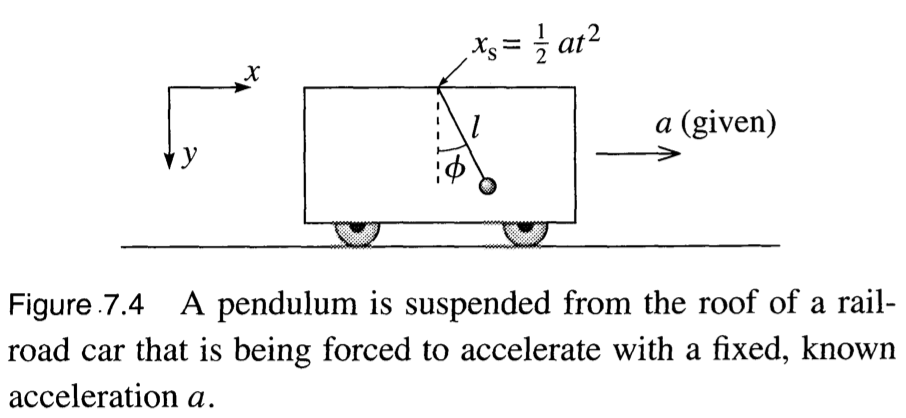
\includegraphics[scale = 0.7]{fig1}\]
\item Find the equilibrium angle $\phi$ at which the pendulum can remain fixed (relative to the car) as the car accelerates. Use the equation of motion to show that this equilibrium is stable. What is the frequency of small oscillations about this equilibrium position? (We shall find a much slicker way to solve this problem in Chapter 9, but the Lagrangian method does give a straightforward route to the answer.)

\end{enumerate}
\end{problem}
\vspace{-0.45cm}
\end{problem}

\begin{solution}

\vfill
\end{solution}

\newpage 

\begin{problem}[ii]
An examination of the relationship between stable equilibria and potential energy minima.

\begin{problem}[7.47]
In Chapter 4 (at the end of Section 4.7) I claimed that, for a system with one degree of freedom, positions of stable equilibrium "normally" correspond to minima of the potential energy $U(q)$. Using Lagrangian mechanics, you can now prove this claim. 
\begin{enumerate}[(a)]
\item Consider a one-degree system of $N$ particles with positions $\vec{ r}_\alpha = \vec r_\alpha(q)$, where $q$ is the one generalized coordinate and the transformation between $r$ and $q$ does not depend on time; that is, $q$ is what we have now agreed to call "natural." (This is the meaning of the qualification "normally" in the statement of the claim. If the transformation depends on time, then the claim is not necessarily true.) Prove that KE has the form $T = \half A \dot q^2$, where $A = A(q) > 0$ may depend on $q$ but not on $\dot q$. [This corresponds exactly to the result (7.94) for $n$ degrees of freedom. If you have trouble with the proof here, review the proof there.] Show that the Lagrange equation of motion has the form 
\[	A(q) \ddot q = -\frac{d U}{d q} - \half \frac{d A}{d q} \dot q ^2 \]
\item A point $q_0$ is an equilibrium point if, when the system is placed at $q_0$ with $\dot q = 0$, it remains there. Show that $q_0$ is an equilibrium point if an only if $dU/dq = 0$. 
\item Show that the equilibrium is stable if and only if $U$ is minimum at $q_0$. 
\item If you did Problem 7.30, show that the pendulum of that problem does not satisfy the conditions of this problem and that the result proved here is false for that system.
\end{enumerate}
\end{problem}
\end{problem}

\begin{solution}

\vfill
\end{solution}


\newpage

\begin{problem}[iii]
The Lagrangian of a system is not unique.\\
\hfill\\
\begin{problem}[7.48]
Let $F = F(q_1, \cdots , q_n)$ be any function of the generalized coordinates $(q_1, \cdots, q_n)$ of a system with Lagrangian $\Lagr(q_1, \cdots, q_n, \dot q_1, \cdots, \dot q_n, t)$. Prove that the two Lagrangians $\Lagr$ and $\Lagr' = \Lagr+ d F/ dt$ give exactly the same equations of motion.
\end{problem}
\vspace{-0.45cm}
\end{problem}

\begin{solution}

\vfill
\end{solution}


\newpage

\begin{problem}[iv]
Lagrange's equations for a system subject to a $\mathbf{B}$ field. Woo-hoo!\\
\hfill\\
\begin{problem}[7.49]
Consider a particle of mass $m$ and charge $q$ moving in a uniform constant magnetic field $\mathbf{B}$ in the $z$ direction. 
\begin{enumerate}[(a)]
\item Prove that $\mathbf{B}$ can be written as $\mathbf{B} = \nabla \times \mathbf{A}$ with $\mathbf{A} = \half \mathbf{B} \times \vec r$. Prove that in cylindrical polar coordinates, $\mathbf{A} = \half B \rho \hat \phi$. 
\item Write the Lagrangian (7.103) in cylindrical polar coordinates and find the three corresponding Lagrange equations. 
\item Describe in detail those solutions of the Lagrange equations in which $\rho$ is a constant.

\end{enumerate}
\end{problem}
\vspace{-0.45cm}
\end{problem}

\begin{solution}

\vfill
\end{solution}

\end{document}
